\documentclass{article}
\usepackage{geometry}
\usepackage{arxiv}
\usepackage[numbers]{natbib}
\usepackage[utf8]{inputenc} % allow utf-8 input
\usepackage[T1]{fontenc}    % use 8-bit T1 fonts
\PassOptionsToPackage{hyphens}{url}\usepackage{hyperref}
\hypersetup{
    colorlinks=true,
    linkcolor=black,
    citecolor=black,
    filecolor=black,      
    urlcolor=black,
    pdftitle={Beat the Bookie},
    breaklinks=true,
    pdfpagemode=FullScreen,
}
\usepackage{booktabs}       % professional-quality tables
\usepackage{amsfonts}       % blackboard math symbols
\usepackage{nicefrac}       % compact symbols for 1/2, etc.
\usepackage{microtype}      % microtypography
\usepackage{lipsum}
\usepackage{glossaries}
\usepackage{graphicx}
\newcommand{\sw}[1]{\texttt{#1}}
% \makeglossaries
\newacronym{ml}{ML}{machine learning}
\newacronym{epl}{EPL}{English Premier League}
\newacronym{rf}{RF}{random forest}
\newacronym{pca}{PCA}{principal component analysis}
\newacronym{lda}{LDA}{linear discriminant analysis}
\newacronym{tsne}{TSNE}{t-distributed stochastic neighbor embedding}
\newacronym{rbf}{RBF}{radial basis function}
\newacronym{umap}{UMAP}{uniform manifold approximation and projection}
\newacronym{mds}{MDS}{multidimensional scaling}
\newacronym{svm}{SVM}{support vector machine}
\newacronym{nn}{NN}{neural network}
\newacronym{lstm}{LSTM}{long short-term memory}
\newacronym{gru}{GRU}{gated recurrent unit}
\newacronym{rnn}{RNN}{recurrent neural network}
\newacronym{cnn}{CNN}{convolutional neural network}
\newacronym{nb}{NB}{Naïve Bayes}
\newacronym{roc}{ROC}{receiver operating characteristic}
\newacronym{lr}{LR}{logistic regression}

\title{Beat the Bookie}


\author{
 Group Name: \texttt{Team C}\\
%  Mohammad Ali Syed, Abdul Al-Fahim, Dylan Hoi, Henry Chen, Chris Wong & Yolanne Lee
  Department of Computer Science\\
  University College London\\
  London, WC1E 6BT\\
}

\begin{document}
\maketitle
%\begin{abstract}
%\lipsum[1]
%\end{abstract}
\vspace{-2em}
\section{Introduction}
\label{intro}
It has long been the ambition of man to take the gamble out of gambling, but alas without any success. However, the recent availability of large-scale data and sophisticated \gls{ml} algorithms may provide a way to at last beat the Bookmakers. No wonder the popularity of attempts to successfully predict sports outcomes has seen a sharp increase in recent years \cite{horvat2020use}.  

In this project, we will attempt to predict the outcome of \gls{epl} matches. Research has shown that football is a very difficult sport to predict given that it is team based, has 3 possible outcomes and goal scoring is sparse \cite{horvat2020use}. Furthermore, past attempts to predict \gls{epl} matches such as \cite{knoll2020machine, teli2018prediction}, vary drastically in methodology and results obtained. Many, such as \cite{owramipur2013football}, also claimed to achieve extremely high accuracy, over 90\%, though these were proven to be unreliable due to their testing process. Indeed, research on predicting football outcomes is extremely nonuniform and yielded no solid foundation on which to approach the problem in a single, decisive manner \cite{horvat2020use}. This problem demanded careful examination and a suitable approach to not only gain good results, but also reliable results. 

Through domain knowledge and analysing previous literature on this topic, we made informed decisions on each stage of this project. Data analysis, as well as our own contextual understanding of the problem task, was combined with sophisticated data transformation techniques to produce a novel, high quality dataset. Multiple classes of cutting-edge \gls{ml} algorithms and suitable model selection techniques were employed to find the best model for our data. By the end of the project, we were able to match the predictive power of the Bookmakers, achieving 52.7\% with a \gls{cnn}.  

The paper adopts the following structure: we will first describe our exploration of the data as well as the transformations applied to it (Section \ref{data}), followed by an overview of our \gls{ml} methodology (Section \ref{methodology}) and a more detailed discussion surrounding \gls{ml} model training and validation (Section \ref{model}). Our results are then analysed in Section \ref{results} and our predictions on the test set given in Section \ref{finalpred}. We conclude our research and avenues for future research in Section \ref{conclusions}.  
\section{Data Transformation and Exploration}
\label{data}
\subsection{Data Analysis}
\label{analysis}
Any \gls{ml} projects requires a granular understanding of the data at hand as well as a contextual understanding. 

We first computed ‘Summary Statistics’, a total of all the existing features as well as the win/loss/draw ratio for each team. Much of the information was unsurprising; those who scored more goals, had more shots on target etc performed better. Interestingly, some teams performed better with fewer goals: Man United had a higher win rate than Arsenal even though Arsenal had scored more goals. Arsenal outperformed Man United on most statistics barring the odd few, most notably the total number of fouls (where Man United had more fouls than Arsenal). This suggested that the more aggressive the team is, the more likely they are to win. It also showed that win rate isn’t wholly determined by number of goals scored as one might naively think. 

\begin{figure}[!htb]
    \centering
    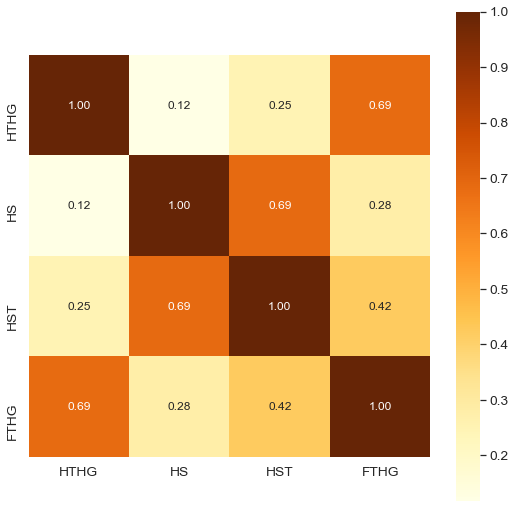
\includegraphics[width=0.5\linewidth]{Images/Figure 1.png}
    \caption{Correlation matrix for \sw{FTHG}s.}
    \label{fig:correlationmatrix}
\end{figure}

We then analysed the correlation matrix for \sw{FTHG} compared to other features (Figure \ref{fig:correlationmatrix}). Unsurprisingly, the highest correlated features were \sw{HTHG}, \sw{HST} and \sw{HS} (same for \sw{FTAG}). This informed our decisions on what custom features to engineer (see below).

\subsection{Feature Selection and Importance Analysis}
\label{featureselection}

Past research has shown that feature selection is an important part of the process and has been shown to boost model performance \cite{horvat2020use}. We therefore wanted to explore the impact and perform feature selection. Mainly, this was all the features except ‘giveaway’ features – features who revealed the winner such as \sw{FTHG}. Before fitting a model, we one hot encoded the \sw{Team Names} and \sw{Referee} features. Dates were split into year, month, week and day as required. However, year was removed since we needed to predict future data; there would be no data with a future year (such as 2022 which is the year for data in the test set) hence hindering performance for future predictions. Labels were label encoded and the data was split into train and test sets of size 70\% and 30\% respectively.  

We chose \gls{rf} as the model to explore feature importance and perform feature selection. \gls{rf} not only produced fruitful results for past projects \cite{horvat2020use}, but it also had useful attributes such as gini impurity \cite{dubeymediumrandomforest} which would allow us to clearly analyse the impact of different features. This would help us gain a better understanding of our data and inform our decisions when it came to feature engineering. Furthermore, it meant further data pre-processing, such as scaling, was not required which saved time. Additionally, it was a model that could easily be visualised, making it easier to interpret and assess how features were impacting the outcome. Model performance on all the features was 56.6\%.  

The first feature we wanted to assess was \sw{Referee}. Given that referees should be unbiased, this feature should be unnecessary. After removing Referee, model performance increased by 0.25\% to 56.89\%. Although the change is marginal, it shows that \sw{Referee} was a noisy feature and hence we removed it before doing feature analysis. This also had the advantage of preventing the curse of dimensionality, given that one hot encoding \sw{Referee} produced over 40 features. The second feature requiring inspection was dates, a random variable that does not have a visible impact on a game. Interestingly, removing dates decreased the accuracy. We therefore decided to keep it for the time being. This provides an interesting area for future research, namely which non-game related features can impact accuracy. 

Having tested non-team related features, we then decided to test \gls{rf} on only the in-game stats. The idea was to see which in-game statistics would be most important if we had access to any of them. We also wanted to remove any noisy in-game stats to produce a purer feature set and inform our decisions for feature engineering. Given the number of features and that they are all correlated, we employed a more advanced technique for feature selection here to judge the most important features. The accuracy on all in-game states was 55.51\%.

\begin{figure}[!htb]
    \centering
    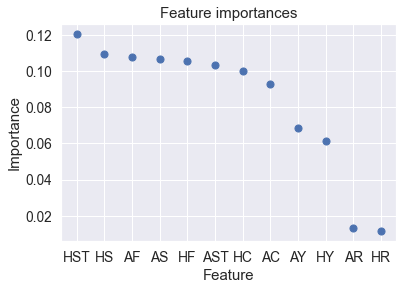
\includegraphics[width=0.5\linewidth]{Images/Figure 2.png}
    \caption{Calculated importance of features }
    \label{fig:featureimportance}
\end{figure}
\vspace{-0.8em}

Feature selection was done using \sw{recursive feature elimination (RFE)}, a ‘wrapper’ method which recursively prunes less important features through a ranking process, using the \gls{ml} model accuracy as a metric. This method was chosen over other options such as \sw{SelectFromModel} due to its superior optimisation iteration process. Other options were also considered such as \sw{Univariate Selection} using \sw{SelectKBest} but were not used due to the extra parameters these methods have which would then need to be tuned \cite{ippolitomediumfeatureselection}. The top 8 features returned by \sw{RFE} were \sw{HST}, \sw{HS}, \sw{AF}, \sw{AS}, \sw{HF}, \sw{AST}, \sw{HC}, \sw{AC}. The reduced feature set produced an accuracy of 54.92\%, a small decrease of -0.58\% compared to using all in-game stats. The reduced feature subset had an interesting effect on the classifications. Precision and recall increased for \sw{Draw}, was unaffected for \sw{Away Win}, but decreased for \sw{Home Win}. This suggests different features are more useful for predicting certain outcomes, an interesting area for future research.

\begin{figure}[!htb]
    \centering
    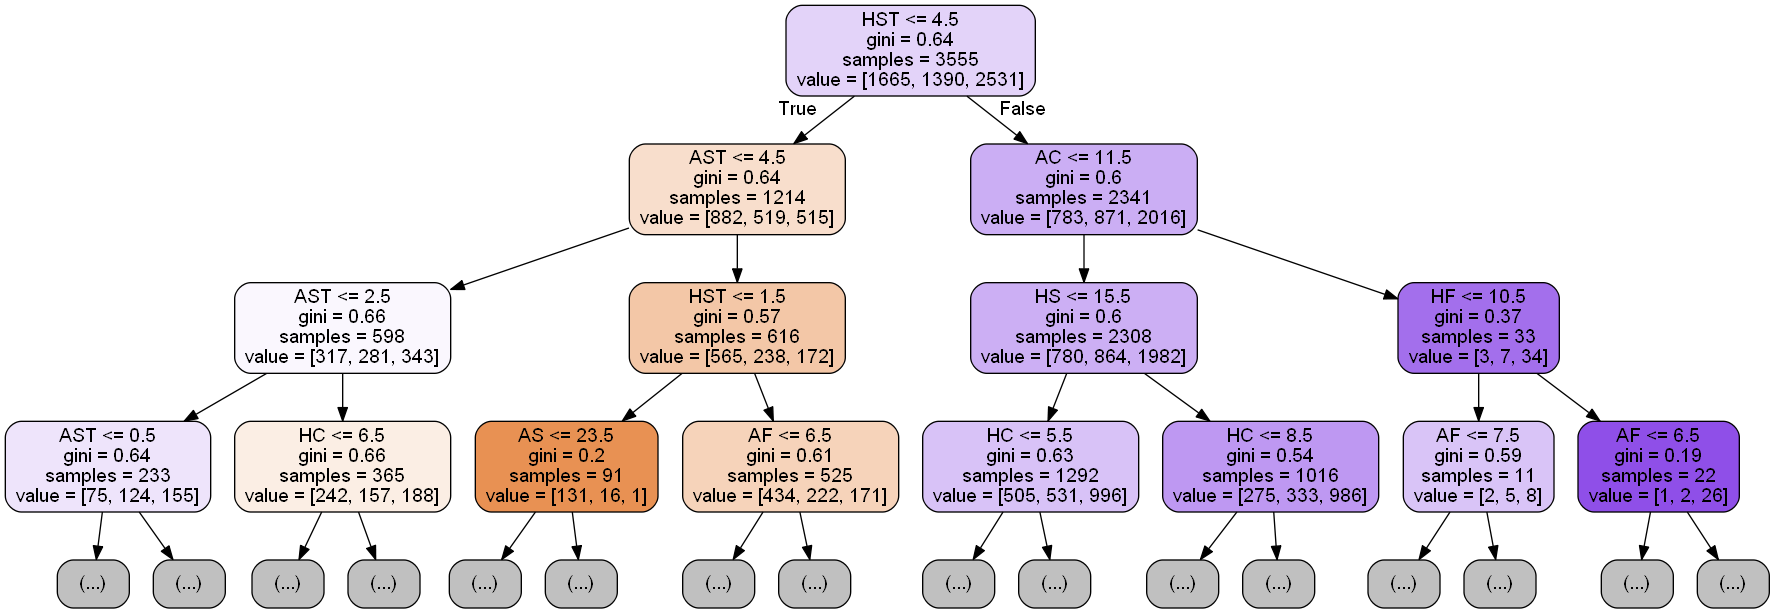
\includegraphics[width=\linewidth]{Images/Figure 3.png}
    \caption{Sample tree displaying how features are used within random forest model.}
    \label{fig:sampletree}
\end{figure}

The different feature importances given by the \gls{rf} model are shown in Figure \ref{fig:featureimportance}, showing a steep decline in importance towards the right. A sample tree from the model was used to visualise how the features were being used by the model and is shown in Figure \ref{fig:sampletree}. 

\subsection{Feature Engineering and Data Collection}
\label{featureengineering}

After gaining a better understanding of the data and using our own intuition of the problem task, we were able to make informed decisions about what custom features to compute. Firstly, we wanted to compute goals / shots on target. This would give us an idea of the skill and scoring strength of the team. For example, a team may have many shots on target, but this is of no use if they are unable to score. Secondly, we wanted to compute shots on target / total shots as this would give the accuracy of a team. Thirdly, given that fouls is an important feature, we decided to compute the ratio of the home teams fouls in the past $k$ matches to away team fouls in the past $k$ matches. This would help assess which team is more aggressive. Finally, we wanted to compute second half goals scored as currently we only had first half goals scored. We believed the second half was a very important aspect of the match, perhaps even more important than the first half, given that mistakes in the first half can be remedied in the second half but not vice versa. We therefore computed second half goals scored for home and away teams. In addition, we computed the previous matches played, goals conceded, win/loss ratio and cumulative goals scored difference.

Beyond the existing features and those we engineered ourselves, we also wanted to obtain any other relevant data from further sources. Past research has found players attributes, team ratings, attack strength, manager performance streak, managers win etc to be effective features \cite{fialho2019predicting, bunker2019machine}. We were able to find several such features including possession, shooting, team ratings and more from various sources \cite{fbref,whoscored}. However, the data was incomplete, going back to only 2017, resulting in the dataset having many missing values. Techniques do exist to impute missing data; however, given that predicting \gls{epl} matches is temperamental at best and previous research suggests features should be limited to only the most effective \cite{horvat2020use}, we decided not to use this data. Furthermore, little research has been done on the best way to handle missing data specifically for sports data. However, we were able to find one extra feature without missing data – distance travelled by the Away team \cite{Kampscshmidtrepo}. The ‘Home Advantage’ is a well-known phenomenon in football \cite{horvat2020use}. Several reasons exist as to why this might be, one of them being fatigue caused by travelling. It therefore stands to reason that the further the distance, the further the fatigue. Hence we believed this could be a useful feature.

Once we had obtained all the required data, we computed prior statistics. In summary, this was the cumulative score for every feature given the past $k$ matches going back to the start of our dataset. This was needed given that for future matches, we would not have access to in-game stats. However, as our dataset would now give historical team strength, it gave little indication as to how strong the team has recently been playing. To provide some balance, we also computed the results and the average shots on goal in the past 3 matches. Finally, the first season of data was removed. This was because to compute the priors, initial matches had stats of 0 which provided no value to the dataset and only added noise. Instead of just removing these initial few rows, we removed the entire first season so that our data began with stats computed using an entire season which we believed would be a more stable dataset for our models to work with. 

We now had an extensive, clean dataset with 38 features known to increase performance from past research. We believed this to be a powerful, high-quality dataset which would produce strong results. 

\subsection{Final Data Pre-Processing}
\label{finaldata}

Given that we would be fitting our data using models other than \gls{rf}, certain pre-processing steps were required which we didn’t do before (as they weren’t required with \gls{rf}).  

Firstly, dates could not be left as the standard numerical values as the models would assume that a higher date (bigger number) is better where this is not true. Instead of one-hot encoding them, research revealed a better option was to model them as sinusoids \cite{kumarmediumonehot}. Not only does this prevent an exponential increase in dimensionality, it allows our models to pick up on cyclic trends that may be present such as team performance dropping near the end of every season due to fatigue from the previous matches. This was prudent given that we saw earlier dates positively affect model performance.

Data was split into train, test and validation set using a ratio of 70\%, 15\%, 15\% respectively. Shuffling was disabled to ensure the order of data was preserved which is very important for time series data \cite{horvat2020use}. However, this does increase the risk of overfitting as there is less randomness in the data. Stratification was not used given that the proportion of each outcome was roughly the same in all segments (45\%, 30\%, 25\% for Home, Away and Draw respectively).  

A separate validation set was used as opposed to k-fold cross validation for the same reason of preserving data ordering and therefore maintaining reliability in validation \cite{horvat2020use, fialho2019predicting}.  

To prevent overfitting on the validation set, we gathered further data going back to 2000 from \cite{footballdata}, increasing the size of the validation set. Combined with using a suitably small function class during model selection, this should mitigate overfitting. 

After scaling the data, dimensionality reduction was employed. Although we only had 38 features strictly speaking, our dataset had 120 features due to one hot encoding team names. Past work has revealed the best results are obtained with a small number of features \cite{horvat2020use}. Dimensionality reduction was used for this rather than feature selection as it allows us to preserve the majority of the information despite the reduction process. A variety of techniques were researched and considered including \gls{pca}, Kernel \gls{pca}, \gls{lda}, and \gls{tsne} \cite{pramodithamediumdimensionality}. We found \gls{pca} was not effective given that the data is not linearly separable. \gls{lda} was also not effective, since it can only find 2 components for our data (given there are only 3 class labels) and is most suited to data that is normally distributed. \gls{tsne} was not suitable for our purposes since it is most effective on data with less than roughly 50 features. Kernel \gls{pca}, however, with the \gls{rbf} kernel and a default sigma of 1/120 (1/number of features), proved effective, since it transformed the data into a higher dimensional space (making it linearly separable) before applying standard \gls{pca}. We chose to reduce the data to 15 features since previous research has shown this to be an optimal choice \cite{horvat2020use}. Further options such as \gls{umap}, Isomap and \gls{mds}, \cite{sivarajahmediumdimensionality} as well as combinations of techniques such as \gls{pca} followed by \gls{tsne}, were also explored but did not produce optimal results.

Finally, some models required categorically encoded labels. 

\section{Methodology Overview}
\label{methodology}

We aimed to test the latest \gls{ml} models most suited to the task at hand to ensure optimal accuracy was achieved. Many past papers use simple \gls{ml} models such as \gls{lr}, \gls{svm} and \gls{nb} \cite{knoll2020machine, teli2018prediction} with good results. Newer research, however, has moved in a different direction. Some papers \cite{tax2015predicting, buursma2011predicting, hucaljuk2011predicting, raju2020predicting} as well as many top Kaggle submissions \cite{kaggleuddinmatchprediction}, make use of boosting algorithms which continuously train weak learners sequentially to correct the mistakes of their predecessor until a learner with sufficient accuracy is built \cite{souzamediumquickguideboosting}. These have proven to be more effective.  

Most papers, however, are now moving towards \gls{nn}s \cite{horvat2020use}. \gls{nn}s have seen many advancements in recent years. Architectures have been developed for time series data, such as \gls{rnn}s. These have an “internal memory” that can remember previous inputs which is ideal for our task \cite{dongesbuiltinRNN}. \gls{rnn}s have also evolved into \gls{lstm}s and \gls{gru}s which help overcome the vanishing gradient issue \gls{rnn}s have \cite{dongesbuiltinRNN}, with several papers utilising \gls{lstm}s successfully \cite{goddijn2018surebet, jain2021soccer}. Another popular \gls{nn} which is not traditionally used for time series data are \gls{cnn}s. However, they have been proven to be rather effective at time series data, due to their innate pattern detection abilities and robustness to noise \cite{brownleemediumconvolutional}. Using \gls{cnn}s for time series data is a growing field and active area of research. 

Finally, we have recently seen the rise of time series models such as \sw{Prophet}. These models are good for predicting seasonal trends, and hence a natural fit for our task. Research surrounding them for sports predictions is limited due to their recent invention, but some recent work with them have found relative success \cite{nandakumarmediumforecasting}. 

Therefore, we decided to test several classes of \gls{ml} models which we believed would provide promising results. These consist of Boosting (\sw{XGBoost}, \sw{AdaBoost}, \sw{GradientBoost}, \sw{LightGBM}), \gls{nn} (Vanilla \gls{nn}, Deep \gls{nn}, \gls{rnn}, \gls{lstm}, \gls{gru}, \gls{cnn} – created with \sw{Keras}) and Time Series (\sw{Prophet}, \sw{Arima}) models. These would be compared to “Base Models” (\gls{lr}, \gls{svm}, \gls{nb}) which would act as the benchmark. In total, we evaluated 15 \gls{ml} models spanning 4 classes (including Base Models as a single class). Our final approach used our \gls{cnn} model since it had the highest accuracy.

Our steps for training and evaluation were the following. Firstly, model selection was done using \sw{Optuna} with a suitable function class on the validation set. Optimal parameters were then used for the \gls{cnn} which fitted on our training set. The model was evaluated using classification accuracy on the test set. 

\section{Model Training and Validation}
\label{model}

\subsection{Model Selection}
\label{modelselection}

Traditionally, \sw{gridsearch} has been a popular and well-known option for hyperparameter tuning. However, research into this area of \gls{ml} exposed \sw{gridsearch} to be severely outdated, ineffective and inefficient compared to its newer counterparts \cite{hyperparamreview}. These packages, such as \sw{hyperopt}, provide significant improvements including providing several ways to search the hyperparameter space such as modified tree parzen estimators \cite{hyperopt}. We decided to use \sw{Optuna} owing to its sophisticated hyperparameter search toolbox (which included \sw{hyperopt}) as well as universal compatibility which was important for us given the number of \gls{ml} models we tested \cite{optuna}.  

The hyperparameter search space was evaluated on our validation set, which contained roughly 3 seasons worth of data. The function class for each model was restricted to prevent overfitting. For the \gls{cnn}, we tested different numbers of nodes (ranging from 32 to 256), sigmoid or softmax activation functions and 4 different optimizers (Adam, Rmsprop, Adagrad, SGD) as these were some of the most important hyperparameters \cite{laumediumCNNtuning}. In particular, a good optimizer is very important to ensure the models is trained optimally. Although Adam is overall a very good optimizer given its use of momentum and adaptive learning rate, it is not always the best, hence the need to test several optimizers. The \sw{Optuna} ‘\sw{study}’ was set to maximise the classification accuracy as this was what we would evaluate our model by on the test set. 

\addtolength{\headsep}{-5mm}
\subsection{Model Training}
\label{modeltraining}

\vspace{-0.6em}
The \gls{cnn} was trained on our training set consisting of roughly 13 seasons worth of data which past research indicated would be more than sufficient \cite{horvat2020use}. The model was trained by using the built in \sw{fit} method for 20 epochs with the Adam optimizer and the default learning rate of 0.001. Categorical cross entropy was used as the loss function.

\vspace{-0.6em}
\subsection{Model Evaluation}
\label{modeleval}

\vspace{-0.6em}
The final model was evaluated using classification accuracy on the test set. This was used as it was an easily interpretable measure that provided a sufficient way to compare models (given that the dataset is not severely imbalanced). Furthermore, this is widely used in past research \cite{horvat2020use}, hence allowing us to easily compare our results in the next section. Other evaluation metrics were considered, for instance logarithmic loss which penalises false classifications and F1 score which combines precision and recall. However, classification accuracy was used for the reasons aforementioned \cite{mishramediummetrics}. 

\vspace{-1.1em}
\section{Results}
\label{results}

\vspace{-0.6em}
\subsection{Optimal Model Analysis}
\label{optimalmodel}

\vspace{-0.6em}
Our best model was our \gls{cnn}, consisting of a single \sw{conv1d} hidden layer with 32 nodes with sigmoid activation and optimized using Adam. This model was able to achieve a high accuracy of 52.7\%, very close to the gold standard of 53\%. It's training and validation accuracies were very close to the test accuracy, indicating the model was trained well and is able to generalise.

\vspace{-1em}
\begin{figure}[!htb]
    \centering
    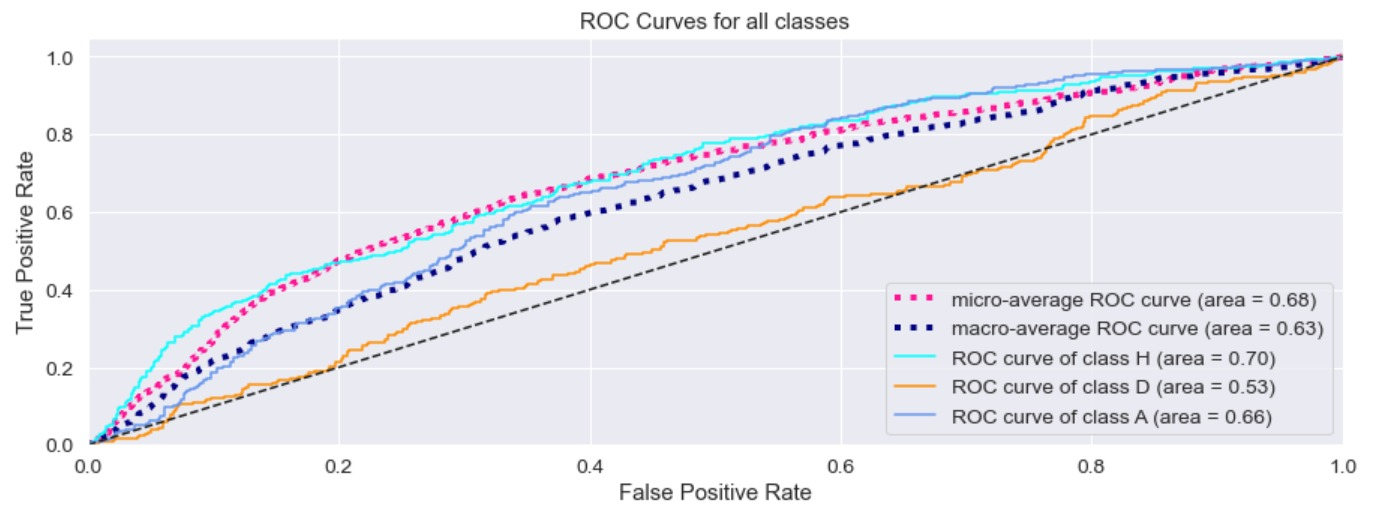
\includegraphics[width=0.9\linewidth]{Images/Figure 4.jpeg}
    \vspace{-0.9em}
    \caption{ROC curve comparison across classes.}
    \label{fig:ROC}
\end{figure}

\vspace{-1em}
\begin{figure}[!htb]
    \centering
    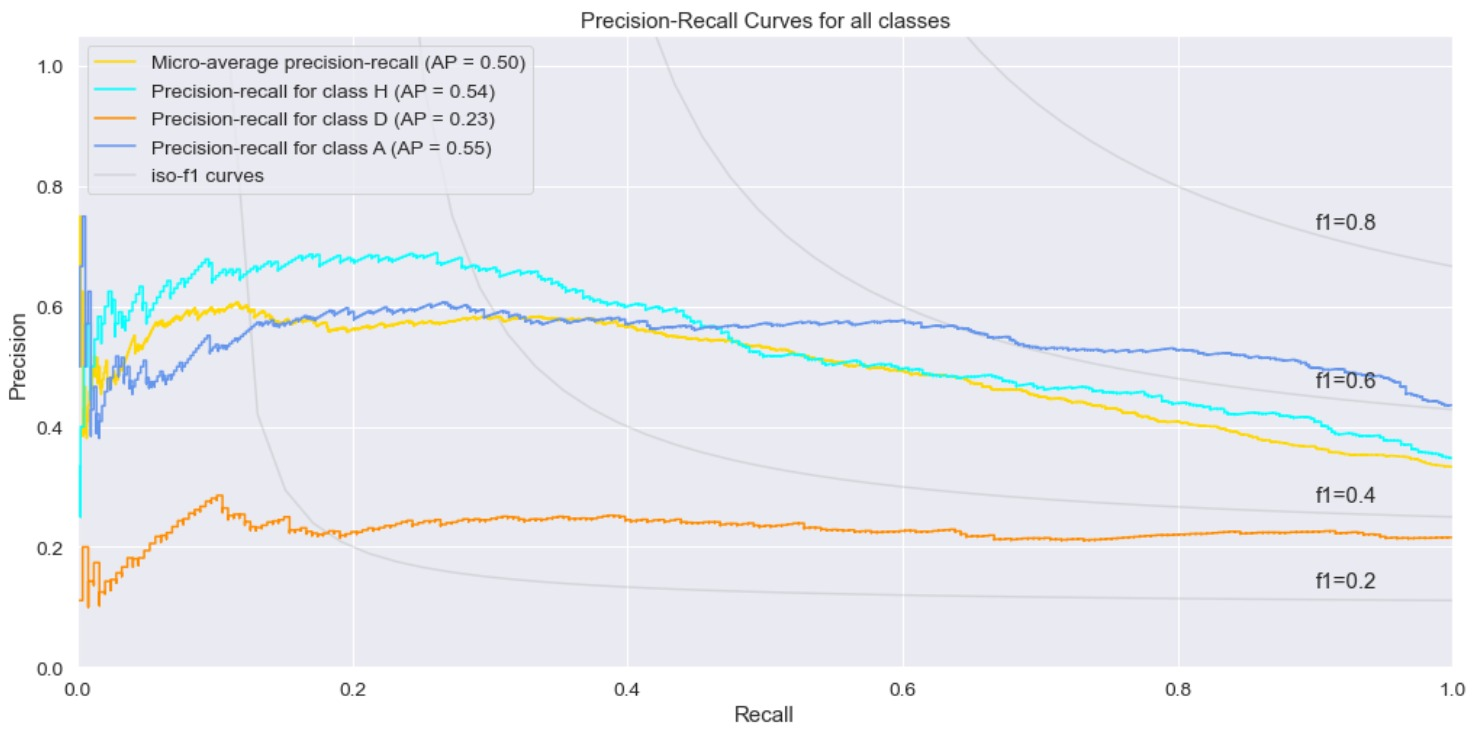
\includegraphics[width=0.95\linewidth]{Images/Figure 5.jpeg}
    \vspace{-0.9em}
    \caption{Precision-recall curve comparison across classes.}
    \label{fig:precisionrecall}
\end{figure}

\subsection{Model Comparison} 
\label{modelcomparison}

% \vspace{-1em}
\begin{figure}[!htb]
    \centering
    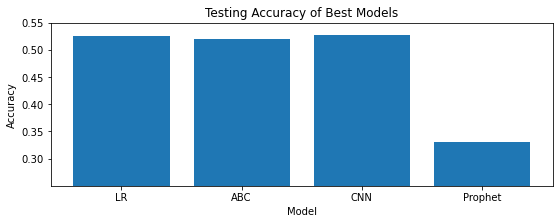
\includegraphics[width=0.7\linewidth]{Images/Figure 6.png}
    \caption{Comparison of test accuracy across models.}
    \label{fig:models}
\end{figure}

Analysing the model’s predictions, we can conclude it is good at predicting Home and Away wins but struggles when it comes to Draws. This is shown in the \gls{roc} curve in Figure \ref{fig:ROC} which shows the trade-off between sensitivity and specificity. We can see that categories A and H have a relatively good trade off but Draw lies roughly on the diagonal, showing predictions for Draws are effectively random. This is also reflected in the precision-recall curve (Figure \ref{fig:precisionrecall}), where the higher area for Home and Away wins show higher precision and recall compared to Draws. This is an area for future research, analysing why Draws appear to be so much harder to accurately predict. 

Comparing the top models from each category (Figure \ref{fig:models}), we can make several observations. Firstly, the top Base Model performs very well compared to the more sophisticated algorithms. This suggests that a dataset like ours which is clean and contains useful features can be used with simpler \gls{ml} models without significantly compromising accuracy. This also has the advantage of reduced model selection and training times as well as an easier process of setting up the model rather than creating one from scratch.  

A more interesting comparison of the top models is to compare their Precision, Recall and F1 scores. Figure \ref{fig:modelcomparisons} shows the Precision, Recall and F1-Score of the top model from each class for \sw{Home Win} outcome. Whilst precision and F1-Score are roughly the same for the top 3 models, Boosting algorithms do suffer when it comes to recall. The exact opposite is true for the \sw{Away Win} outcome, however.  

Judging models based on accuracy is not sufficient. Analysing the predictions more thoroughly can allow one to make more informed decisions about choosing a model according to one’s priorities. For instance, if \sw{Away Wins} provides the highest monetary reward in betting, perhaps a model which can accurately predict \sw{Away Wins} would be preferred over an all-rounder. This is an interesting area for future research. 

Analysing the training accuracies does not yield any significant conclusions except that \sw{XGBoost} had a very high training accuracy of roughly 56\%. Given that the other models had roughly the same training and test accuracies, \sw{XGBoost} may have been overfitted slightly. This can be solved by increasing the regularization parameter. 

\subsection{ML Class Comparison} 
\label{classcomparison}

Comparing overall accuracies of each, Boosting models perform the best. This is not surprising given past research has yielded good results with Boosting models. However, the difference is marginal compared to Base Models and NNs. Moreover, as with NNs, Boosting algorithms come with a significant number of hyperparameters which must be tuned carefully. 

Base Models performed surprisingly well considering they are much less sophisticated than the other models. As mentioned above, these models have the advantage of being simpler, faster and more reliable to train. Furthermore, such models are generally easier to visualise through XAI techniques compared to the more advanced ML models. Such techniques could provide key information about how to progress in predicting EPL outcomes. 

It is interesting to see that the RNN, LSTM and GRU, models developed for time series data, do not seem to provide any advantage over their counterparts. This could suggest that perhaps historical team performance doesn't provide significant value, given that these models which are most suited to such a scenario weren't able to make use of it any more than the other models. 

Finally, regarding Time Series models, our results suggest that, while underlying date and time trends may exist in the data (given the accuracy isn’t 0), models which focus too much on this may suffer. We believe a better use of these models would be to use them in combination with another ML model; the main ML model could focus on extracting all possible information from team and game statistics and the Time Series model could then factor in seasonal trends.

\begin{figure}[!htb]
    \centering
    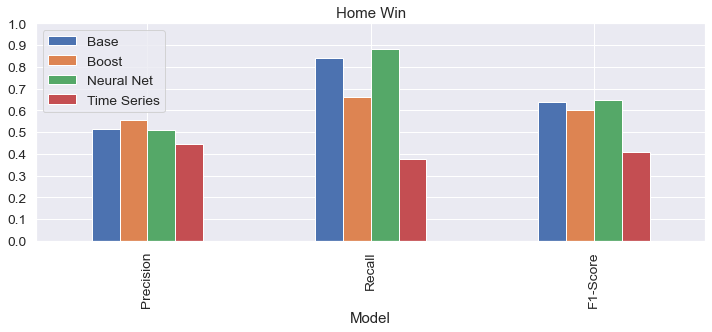
\includegraphics[width=0.7\linewidth]{Images/Figure 7.png}
    \caption{Average precision, recall, and F1 scores across best models in each class.}
    \label{fig:modelcomparisons}
\end{figure}

 

\subsection{Comparison to Past Research}
\label{pastresearch}

Our results seem to be on par with past research, not being significantly higher nor lower. Examples include \cite{goddijn2018surebet} who achieved 51\% using \gls{lstm} and \cite{mccabe2008artificial} who achieved 58.9\%. It was also interesting to note that we achieved roughly the same accuracy as \cite{dubitzky2019open}, even though our feature set was significantly smaller. This supports research that more features don’t necessarily improve accuracy \cite{horvat2020use}.  

Some previous studies obtained extremely high accuracy, such as \cite{owramipur2013football} which achieved over 90\%. These results, however, are unreliable. This paper uses the same data for training and testing, hence such high results are misleading.

Some papers do achieve higher results than ours which seem valid, such as \cite{hucaljuk2011predicting}, however they predict other football leagues such as Champion’s League. Research has shown that predicting different football leagues can yield vastly different results hence comparisons to such papers is unsuitable \cite{horvat2020use}. Therefore, we can conclude that our approach, whilst being different from past research, yields suitable results. 

\section{Final Predictions on Test Set}
\label{finalpred}

\vspace{-1em}
\begin{figure}[!htb]
    \centering
    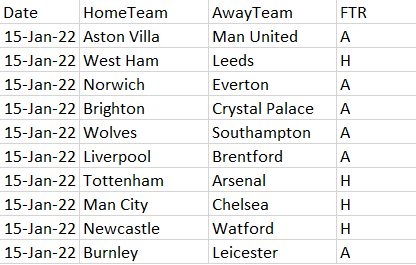
\includegraphics[width=0.45\linewidth]{Images/Figure 8.png}
    \caption{Final predictions on test data.}
    \label{fig:predictions}
\end{figure}

We applied the same feature engineering and data pre-processing on the Test set as we did on the training set, after which we used our trained \gls{cnn} model to make our predictions. Our predictions are shown in Figure \ref{fig:predictions}.

\section{Conclusion and Future Research}
\label{conclusions}

In this project, we aimed to produce a high-quality dataset and apply appropriate \gls{ml} techniques to predict outcomes of \gls{epl} matches, matching the predictive accuracy of the Bookmakers. Through domain understanding, data analysis, feature selection, dimensionality reduction and feature engineering we successfully produced a high-quality dataset going back to 2000. After extensive research of past projects, we were able to shortlist a range of \gls{ml} models of varying sophistication from which we were able to select the top performing model, a \gls{cnn} which was tuned through \sw{Optuna} on our validation set, based on its strong classification accuracy on the test set, matching the accuracy of the Bookmakers.  

Our project has revealed several avenues for future research. Firstly, external features such as weather should be explored for their possible impact on predictions, given that dates affected our accuracy. Secondly, ensemble models provide a way to overcome limitations of individual models to create an all-rounder. This has been fruitful for many top Kaggle submissions such as \cite{lumedium35}. Thirdly, predicting sports outcomes itself is unlikely to be the main aim for individuals or organisations. Custom loss functions can be used to suit the needs of the individual. For example, one project used a custom loss function to maximise the monetary reward from predictions rather than maximise the accuracy \cite{malafossemediumnotclassification}. Other avenues include using NLP to analyse situation specific sentiment which has been shown to boost model accuracy by over 6\%. \cite{beal2021combining}.

\bibliographystyle{unsrtnat}
{\footnotesize
\bibliography{refs}}
\end{document}